\documentclass[a4paper]{article}

%% Language and font encodings
\usepackage[english]{babel}
\usepackage[utf8x]{inputenc}
\usepackage[T1]{fontenc}
\usepackage{caption}

%% Sets page size and margins
\usepackage[a4paper,top=3cm,bottom=2cm,left=3cm,right=3cm,marginparwidth=1.75cm]{geometry}

%% Useful packages
\usepackage{amsmath}
\usepackage{amsfonts}

\usepackage{graphicx}
\usepackage{tikz}
\usetikzlibrary{arrows.meta}

\usepackage[colorinlistoftodos]{todonotes}
\usepackage[colorlinks=true, allcolors=blue]{hyperref}

\usepackage{color}
\usepackage{url}

%% display solutions or not
\newif\ifsol
\soltrue % comment out to hide solutions

%% todo tracker -- overleaf v2 has better one it uses but will default to this if compiled on something that doesn't have built-in todo
%\newcommand{\todo}[1]{\textbf{\textcolor{red}{#1}}}

\title{Exam 1 Compiled Section Notes}
\author{CS 182 - Artificial Intelligence}
\date{}

\begin{document}
\maketitle

\section{Search}
\renewcommand{\labelenumii}{\arabic{enumii}.}
\setlength{\parindent}{0pt}

A \textbf{search problem} can be defined by the tuple
$(S, A, R, C, S_0, G)$, where
\begin{itemize}
\item $S$ represents the set of possible \underline{states}

\item $A$ represents the set of possible \underline{actions}, which may vary
from state to state

\item $R : S \times A \rightarrow S$ is the \underline{transition model},
which represents the result of actions from a state

\item $C : S \times A \rightarrow \mathbb{R}$ represents the \underline{cost}
of taking an action

\item $S_0$ represents the \underline{starting state}

\item $G$ represents the \underline{goal test}, the set of {goal states}
\end{itemize}

Together, these parameters implicitly form a \underline{state space graph},where nodes are possible states and edges are actions connecting states.\\

\underline{Tree search} is a method of exploring a state space graph by expanding out potential plans. Tree search builds a tree of searched states and maintains a \underline{fringe} of partial plans under consideration. The objective is to find a plan that reaches the goal state, and it is ideal to try to expand as few nodes as possible on the state space graph.\\

\underline{Graph search} extends tree search to account for state space graphs with cycles by keeping a set of visited nodes. These visited nodes are not explored again, avoiding repeated work.\\

\textbf{Uninformed Search:}
\begin{itemize}
\item \underline{Depth-First Search ({DFS})} maintains the fringe as a stack. Expands the ``deepest'' nodes first.

\item \underline{Breadth-First Search ({BFS})} maintains the fringe as a queue. Expands the ``shallowest'' nodes first.

\item \underline{Uniform Cost Search ({UCS})} maintains the fringe as a priority queue ordered by the cumulative cost of a path. UCS is optimal for all edge costs $>0$.
\end{itemize}

\textbf{Informed Search:}
\begin{itemize}
\item \underline{Greedy Search }maintains the fringe as a priority queue ordered by a heuristic function $h(x)$ that maps states to estimated distance to goal.

\item \underline{A* Search extends} greedy search and maintains the fringe as a priority queue ordered by summing the cumulative cost of a path to state $x$, $g(x)$, and the heuristic at $x$, $h(x)$ aka
$f(x) = g(x) + h(x)$.
\end{itemize}

\newpage
\noindet Psuedocode for both Tree and Graph search are shown below. Note: the frontier referenced below is the fringe. Think about how using a different data structure for the fringe would allow each of the algorithms to execute the above search algorithms.

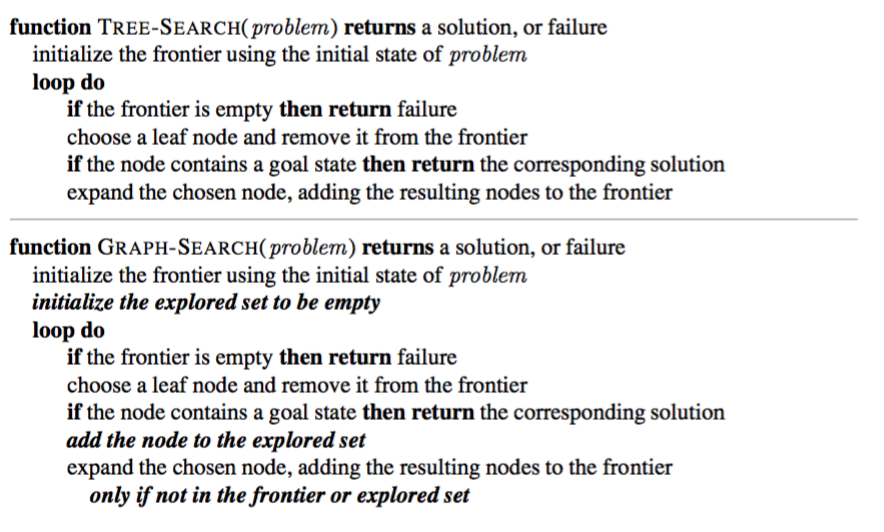
\includegraphics{figs/search}

\textbf{Heuristics:}
\begin{itemize}
\item A heuristic function is used to estimate the cost of reaching a goal from a state.
\item A heuristic $h$ is \underline{admissible} if it never overestimates the cost of reaching the goal, i.e. $\forall x, h(x) \le h^*(x)$ where $h^*$ is the optimal cost to reach the goal.
\item A heuristic $h$ is \underline{consistent} if it never overestimates the estimated distance to the goal of a neighbor plus the cost of reaching the neighbor, i.e. $\forall x, h(x) \le c(x, x') + h(x')$
\end{itemize}

\section{Games}
\noindent Recall the formalization of a \textbf{Deterministic Game} from lecture:
\begin{itemize}
\setlength\itemsep{0.2em}
\item States: $S$ (with start state $S_0$)
\item Actions: $A$ (may depend on player/state)
\item Transition Function: $R:$ $S \times A \rightarrow S$
\item Players: $P=\{1 \ldots N\}$ (usually take turns)
\item Terminal Test: $T:$ $S \rightarrow \{True,False\}$
\item Terminal Utilities: $U:$ $S \times P \rightarrow R$
\end{itemize}

\noindent And that a solution for a player is a policy $\Pi: S \rightarrow A$.
\\ \\
\noindent Note that the difference between a game and a search problem is that introduction of multiple players and their policies and a goal test / terminal utility instead of a cost of actions and a goal state set.
\\ \\ 
\textbf{Minimax:} Recall that in games, every state has a value $V$. For terminal states, $V(s)$ is known. In single-player games, you can calculate the value for non-terminal states as 
$$V(s) = \underset{s' \in \textrm{successors}(s)}{\operatorname{max}} V(s')$$
Now imagine a two-player, zero-sum, turn-based game like Tic Tac Toe. We still know $V(s)$ for terminal states, but now we have to anticipates the opponents' turn. In the minimax algorithm, we assume that the opponent plays rationally and tries to minimize your reward (thus maximizing theirs). Therefore, for your opponents' turns, we calculate the value of a state as 
$$V(s') = \underset{s \in \textrm{successors}(s')}{\operatorname{min}} V(s)$$
Therefore, with two rational agents the optimal strategy is to maximize your moves and assume your opponent will do the same (thus minimizing your utility on their turn), thus minimax. Of course if our opponent isn't optimal, then we can still use this type of procedure if we consider the opponent's move in expectation, thus expectimax!
\\ \\
\textbf{Alpha-Beta Pruning} is an extension of Minimax which increases efficiency by reducing the number of nodes searched. While we traverse the tree, we keep track of two values, $\alpha$, and $\beta$. $\alpha$ is MAX's best solution on the path to root, $\beta$ is MIN's best option on the path to root. We then follow the procedure below allowing us to eliminate the need to search over sections of the tree to which we know will not be a part of the optimal solution.
\begin{figure}[ht]
\centering
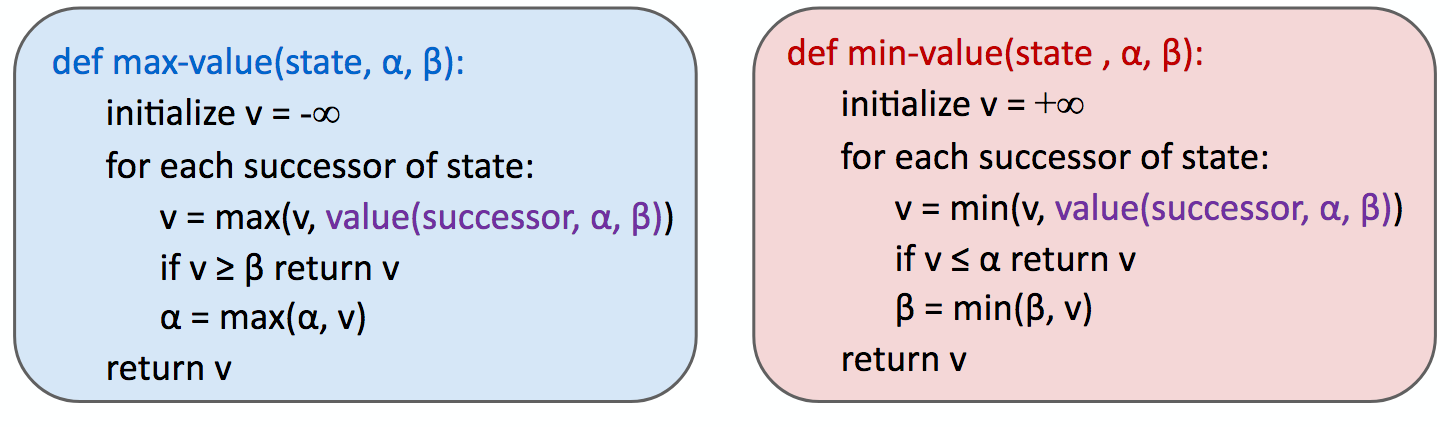
\includegraphics[width=0.7\textwidth]{figs/abalg}
\end{figure}

We can think of alpha-beta pruning as pruning branches of the tree when we know that for sure no better solution could possibly be reached given the zero-sum nature of the game.

\section*{CSPs}
\noindent \textbf{CSPs} are formalized as a triple $\langle X,D,C \rangle$. 
\begin{enumerate}
\item $X = \{X_1, \ldots, X_n\}$: A set of variables in the problem
\item $D = \{D_1, \ldots, D_n\}$: The domains for these variables
\item $C = \{C_1, \ldots, C_m\}$: Constraints
\end{enumerate}
Constraints encode the limits on the values/domains for each variable contingent on the values/domains of other variables.
\\ \\
\noindent One way to solve a CSP is through \textbf{backtracking search} which is simply DFS with two changes:
\begin{enumerate}
\item Fix the variable ordering ($X_1 = D_1 \rightarrow X_2 = D_2 \equiv X_2 = D_2 \rightarrow X_1 = D_1$).
\item Check constraints as you go and backtrack if you violate any.
\end{enumerate}
One way to optimize this process is to use the most constrained variable (the variable with the minimum remaining values) and assign the least constraining variable. Another optimization is to use \textbf{forward checking} to do a one step check for inconsistent solutions at each assignment. Finally one can use \textbf{arc consistency} to check the entire chain of implications of one assignment.\\

Finally to turn a graph into a tree (and then apply tree based CSP algorithms) one can find the minimal \textbf{cutset} which will divide up the graph. Note that this then means that you may need to search over all possible cutset values.

\newpage
\section*{Local Search}
\noindent \textbf{Optimization} is the process of computing an optimal solution (e.g., min cost, max reward) to some mathematical problem. Optimization is often used to solve complex problems as it casts a real world problem into a simple math problem which can be solved via off-the-shelf solvers. Unfortunately, many optimization problems are NP-complete. Therefore, globally optimal solutions cannot often be found and instead locally optimal solutions are searched for from some (ideally) informed initial condition. \textbf{Local Search Algorithms} include:
\begin{enumerate}
    \item \textbf{Hill Climbing} is the simplest approach. Given a state $s$, generate all successors $s'$ and move to the best one. If there is no better successor, return the current state. A variant of this allows for \textbf{random restarts} to try to escape local minimums.
    \item \textbf{Simulated Annealing} picks a random successor state at each step. If the random successor is better, the state moves. If it is worse, it is accepted with probability $\exp(\Delta E / T)$. The algorithm starts with large $T$ (exploration) and decreases it over time. 
    \item In \textbf{Beam Search}, we choose $k$ random initial states. All successors for all $k$ states are expanded. Among all of the generated states, the best $k$ states are chosen. 
    \item \textbf{Genetic Algorithms} start with a set of possible solutions. Inspired by natural selection, at each iteration, a biased sample (based on a measure of ``fitness'') is taken from the current solution set. A new solution set is then constructed by ``crossing over'' (aka combining parts of) pairs of sampled solutions. ``Mutation'' (aka random changes to solutions) are also added during iterations. These algorithms can avoid local minima but may take many iterations to converge to a good solution.
    \item \textbf{Gradient Descent} relies on an assumption that we are minimizing a locally convex (or maximizing a locally concave) function. It takes the gradient, the partial derivatives, of the function which points in the direction of maximum descent (ascent) and moves in that direction iteratively, $x_{t+1} = x_t - \alpha \nabla f(x)$, until it reaches a local minimum (maximum) where $\nabla f(x) = 0$. \textbf{Stochastic Gradient Descent} approximates the gradient through sampling and is otherwise the same. $x_{t+1} = x_t - \alpha \left(f(x+w) - f(x)\right)w$ for $w \sim \mathcal{N}(0,\,\Sigma)$. These are both used in continuous domains.
\end{enumerate}

\section*{MDPs}
\renewcommand{\labelenumii}{\arabic{enumii}.}
\setlength{\parindent}{0pt}

Recall that a \textbf{Markov Decision Process} is defined by
\begin{itemize}
  \item $S$: the set of possible \underline{states}

  \item $A$: the set of possible \underline{actions}, which may vary
  from state to state

  \item $T(s, a, s') \rightarrow \mathbb{R}$:
  the \underline{transition function} is the probability
  that $a$ from $s$ leads to $s'$

  \item $R(s, a, s') \rightarrow \mathbb{R}$:
  the \underline{reward function}. This could also be
  listed as $R(s')$ or $R(s,a)$

  \item The \underline{starting state}, and, potentially, a \underline{terminal state}
\end{itemize}

With MDPs, we want to find the optimal policy $\pi^*: S \rightarrow A$,
which maximizes the expected utility.

Since we need to maximize the expected utility, we need that utility to be finite. We do this by:

\begin{enumerate}
  \item \underline{Choosing a finite horizon}: By terminating the game after $T$ steps the reward must be finite. This often generates nonstationary policies, as $\pi$ depends on time remaining.
  
  \item \underline{Discounting over an infinite horizon}: Multiplying rewards by the discount rate $0 < \gamma < 1$ every time a new step is made will cause the solution to converge to a finite return and thus a finite solution, where a smaller discount rate ($\gamma$) leads to a shorter term focus.
  $$U([r_0, \cdots, r_\infty]=\sum_{t=0}^\infty \gamma^tr_t$$

  \item \underline{Having an absorbing state}: This guarantees that all policies eventually reach a terminal state.
\end{enumerate}

We define a \textbf{Q-state} $Q(s, a)$ as the expected utility of having taken action $a$ from state $s$ and acting optimally afterward:
$$Q^*(s,a) = \sum_{s'}T(s, a, s')[R(s, a, s') + \gamma V^*(s')]$$

And the \textbf{Value} of a state $V(s)$ as the expected utility of starting in $s$ and acting optimally. This can also be thought of as taking the best action $a$ at Q-state $Q(s,a)$:
$$V^*(s) = \max_a \sum_{s'}T(s, a, s')[R(s, a, s') + \gamma V^*(s')] = \max_a Q^*(s, a)$$

\textbf{Value Iteration} is a way to compute the optimal value for every state. It is done by first initializing the values for each state to 0:
$$V_0(S) = 0$$
Then the $k+1$ iteration will take the vector of $V_k(s)$ for all states $s$ and make a one step (Bellman) update:
$$V_{k+1}(s) = \max_a \sum_{s'} T(s, a, s') [R(s,a,s') + \gamma V_k(s')]$$

Unfortunately, this process is quite slow, as while the optimal action at each state (and thus the optimal policy) rarely changes, the optimal values can take many iterations to finally converge. Furthermore, each iteration is $O(S^2A)$ and thus the dimensionality and time complexity of the problem grows quite quickly with the size of the state or action space.

\textbf{Policy Iteration} attempts to overcome these issues by iteratively alternating between \textbf{Policy Evaluation} (updating the values) and \textbf{Policy Improvement} (updating the policy). This both reduces time complexity of the algorithm and allows it to exit earlier once the policy converges.

\textbf{Step 1: Policy Evaluation:} Starting with $V_k^{\pi_k}(s')$ and iterating (over $i$), update the values under a fixed policy $\pi_k$ until convergence:
$$V^{\pi_k}_{i+1}(s) = \sum_{s'} T(s, \pi_k(s), s') [R(s,\pi_k(s),s') + \gamma V_i^{\pi_k}(s')]$$
Call the converged values $V^{\pi_k}_{k+1}(s)$, and use them to update the policy:

\textbf{Step 2: Policy Improvement:} Extract a better policy based on these new values:
$$\pi_{k+1}(s) = \text{arg max}_a \sum_{s'} T(s, a, s') [R(s,a,s')+ \gamma V^{\pi_k}_{k+1}(s')] = \text{arg max}_a Q_{k+1}(s,a)$$

Note that Policy Evaluation is $O(S^2)$ operation and that both steps of Policy Iteration are easier to extract from the Q-values than the Values themselves.

\section*{Reinforcement Learning}
\noindent We use \textbf{Reinforcement Learning (RL)} when we have a Markov Decision Process (MDP) for which we know: 
\begin{itemize}
    \item $S$: set of states
    \item $A$: set of actions (for any given state)
    \item $s_0$: start state
    \item $s_g$: goal state (or set of goal states)
\end{itemize}
but do not know:
\begin{itemize}
    \item $T : S \times A \to S$: transition map (or model)
    \item $R : S \times A \to \mathbb{R}$: reward function
\end{itemize}
\newpage
The goal of reinforcement learning is to learn a \textbf{policy} $\pi: S \to A$ which returns the best action for any given state in the problem. In the process of looking for the policy, RL algorithms often calculate:
\begin{itemize}
    \item $V : S \to \mathbb{R}$: \textbf{value function}, which stores the utility of every state
    \item $Q : S \times A \to \mathbb{R}$: \textbf{Q-value function}, which stores the value of every (state, action) pair \\
\end{itemize}

\noindent In \textbf{Passive Reinforcement Learning}, an agent has a fixed policy, and learns about the environment while executing that policy. In lecture, we discussed two algorithms:
\begin{enumerate}
    \item \textbf{Direct evaluation} runs many "experiments", or "simulations", resulting from following a given policy $\pi$, and keeps track of the total discounted rewards of the visited states. Afterwards, the reward instances for each state are averaged to determine the state's value. This could be written as
    \[
    V(s) = \frac{1}{n} \sum_i (R(s_i) + \gamma R(s_i') + \gamma^2 R(s_i'') + ...)
    \]
    where $s_i$, $s_i'$, $s_i''$, $\dots$, are the states visited in the $i$th simulation. Direct evaluation can also be referred to as a \textbf{Monte Carlo} approach, since it depends on averaging over many randomized simulations or samples.
    \item \textbf{Temporal difference learning} iteratively runs experiments following a given policy. With each transition, a sample-based Bellman update is made to the value of the visited state (both equations are computing the same thing):
    \[
    V^{\pi}(s) \leftarrow V^{\pi}(s) + \alpha [R(s, \pi(s), s') + \gamma V^{\pi}(s') - V^{\pi}(s)]
    \]
    \[
    V^{\pi}(s) \leftarrow (1- \alpha) V^{\pi}(s) + \alpha [R(s, \pi(s), s') + \gamma V^{\pi}(s')]
    \]
    We can think of this algorithm can be thought of as sample-based policy evaluation. Remember policy evaluation was:
    $$V^{\pi}(s) \leftarrow \sum_{s'} T(s, \pi_k(s), s') [R(s,\pi(s),s') + \gamma V^{\pi}(s')]$$
    In Q-learning we are still executing some policy $\pi$ we just don't know what the transition model is and thus can't compute all of the possible transitions to sum over. Instead we are simply computing one of the values in the sum and making a weighted update of our current value to incorporate the new information.
\end{enumerate}

\noindent In \textbf{Active Reinforcement Learning}, and agent chooses actions and tries to find an optimal policy while learning about the environment. The primary algorithm used in active RL is \textbf{Q-learning}. Similarly to TD learning, Q-learning makes sample-based Bellman updates, but to Q-values instead of values:
\[
Q(s, a) \leftarrow Q(s, a) + \alpha [R(s, a, s') + \gamma \max_{a'} Q(s', a') - Q(s, a)]
\]
\[
Q(s, a) \leftarrow (1 - \alpha) Q(s, a) + \alpha [R(s, a, s') + \gamma \max_{a'} Q(s', a')]
\]
Since we are learning Q-values and not values we can extract the current estimate of the optimal policy by doing a one-step argmaximization over the Q-value immediately at any time: \\
\[
\pi(s) = arg\max_{a} Q(s,a)
\]

\newpage
\noindent Some algorithmic details and variations:
\begin{enumerate}
    \item In active algorithms, we must choose actions to take from states. One approach is \textbf{$\epsilon$-greedy action selection}: with (small) probability $\epsilon$, actions are chosen randomly; with (large) probability $1 - \epsilon$, we choose the current optimal action. This encourages exploration of the state space and is generally helpful in practice. Note that this is called off-policy learning as we learn the exact Q-values but execute with a different policy, the $\epsilon$-greedy policy.
    \item How can we evaluate the choice of parameters or exploration functions in Q-learning? One approach is to measure \textbf{regret} -- the difference between expected rewards and final optimal rewards.
    \item In linear \textbf{approximate} (or \textbf{feature based}) \textbf{Q-learning} we approximate the Q-function with a set of functions which are intended to represent higher-level features of the state space: 
    \[
    Q(s,a) = w_1 f_1(s,a) + w_2 f_2(s,a) + \dots + w_m f_m(s,a)
    \]
    For example, for PACMAN they could be the number of ghosts, the distance to the nearest ghost, the distance to the nearest food, etc. The advantage here is that we simply need to learn the correct weights, and thus we have fewer parameters to learn than in standard Q-learning, where we have to learn a table of Q-values for every single state-action pair. The disadvantage is that the quality of the Q-values is highly dependent on the quality of the functions. The update of the weights based on new information is:
    \[
    w_i \leftarrow w_i + \alpha f_i(s,a) [R(s, a, s') + \gamma \max_{a'} Q(s', a') - Q(s, a)]
    \]
    
\end{enumerate}

\noindent Algorithmic parameters:
\begin{itemize}
    \item $\alpha$: learning rate (determines the integration of new information into current estimates)
    \item $\gamma$: discount rate (determines how quickly rewards decay with time)
\end{itemize}
\end{document}